\documentclass{article}
\usepackage[UTF8]{ctex}
\usepackage{pythonhighlight}
\usepackage{markdown}
\usepackage{listings}
\lstset{
    basicstyle          =   \tt,          % 基本代码风格
    identifierstyle=\color{brown!80!black},
    keywordstyle        =   \color{purple}\bfseries,          % 关键字风格
    commentstyle        =   \rmfamily\itshape,  % 注释的风格,斜体
    stringstyle         =   \ttfamily,  % 字符串风格
    flexiblecolumns,                % 别问为什么,加上这个
    numbers             =   left,   % 行号的位置在左边
    showspaces          =   false,  % 是否显示空格,显示了有点乱,所以不现实了
    numberstyle         =   \zihao{-5}\ttfamily,    % 行号的样式,小五号,tt等宽字体
    showstringspaces    =   false,
    captionpos          =   t,      % 这段代码的名字所呈现的位置,t指的是top上面
    frame               =   lrtb,   % 显示边框
    backgroundcolor=\color[RGB]{245,245,244},
}


% Language setting
% Replace `english' with e.g. `spanish' to change the document language
\usepackage[english]{babel}
\usepackage{float}
% Set page size and margins
% Replace `letterpaper' with `a4paper' for UK/EU standard size
\usepackage[letterpaper,top=2cm,bottom=2cm,left=3cm,right=3cm,marginparwidth=1.75cm]{geometry}

% Useful packages
\usepackage{amsmath}
\usepackage{graphicx}
\usepackage[colorlinks=true, allcolors=blue]{hyperref}

\title{数逻实验报告Lab11}
\author{雷远航}

\begin{document}

\maketitle

\begin{abstract}
    寄存器和寄存器传输设计
\end{abstract}

\section*{一、操作方法与实验步骤}
\subsection*{任务:基于ALU的数据传输应用设计}
\subsubsection*{完成top.v文件的设计}
根据实验的要求,完成top.v,实现各种模式下的ALU运算,以及寄存器传输的操作,
使其具备全部的功能.

top.v的完成如下:
    \begin{figure}[H]
    \centering
    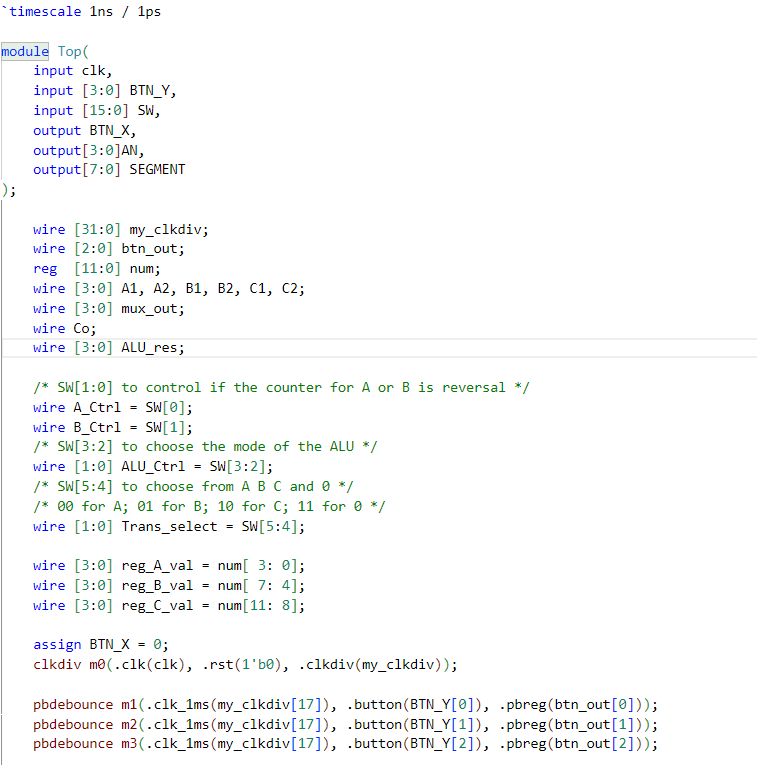
\includegraphics[width=0.7\textwidth]{1.png}
    \caption{\label{Lab11}top.v}
    \end{figure}


    \begin{figure}[H]
    \centering
    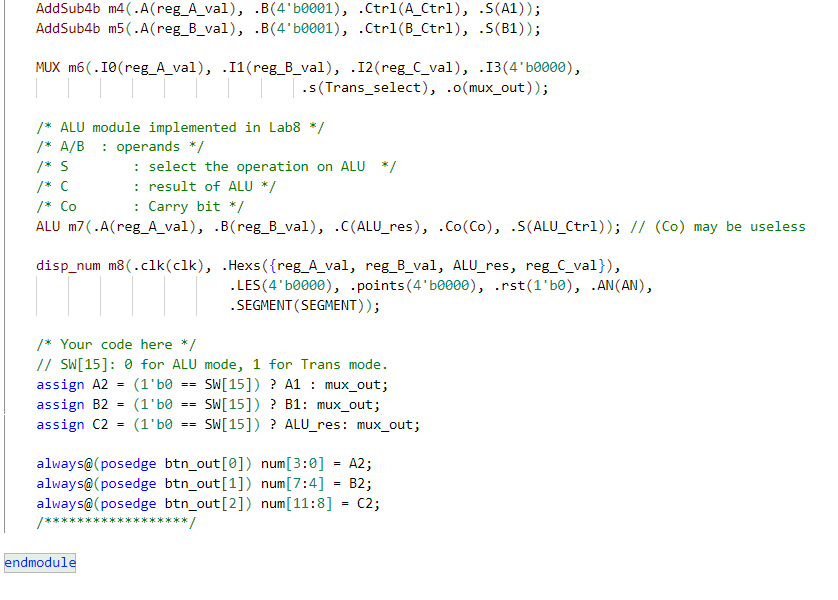
\includegraphics[width=0.7\textwidth]{2.png}
    \caption{\label{Lab11}top.v}
    \end{figure}

\subsubsection*{完成全部的工程}
导入前面实验已经完成的时钟模块、防抖动模块、数字显示模块,从而完成全部的工程,
然后进行下版验证.

\section*{二、实验结果与分析}
\subsection*{下版验证与分析}

\subsubsection*{ALU运算模式:}
拨动开关使得SW[15]的信号为0,进入ALU运算模式
    \begin{figure}[H]
    \centering
    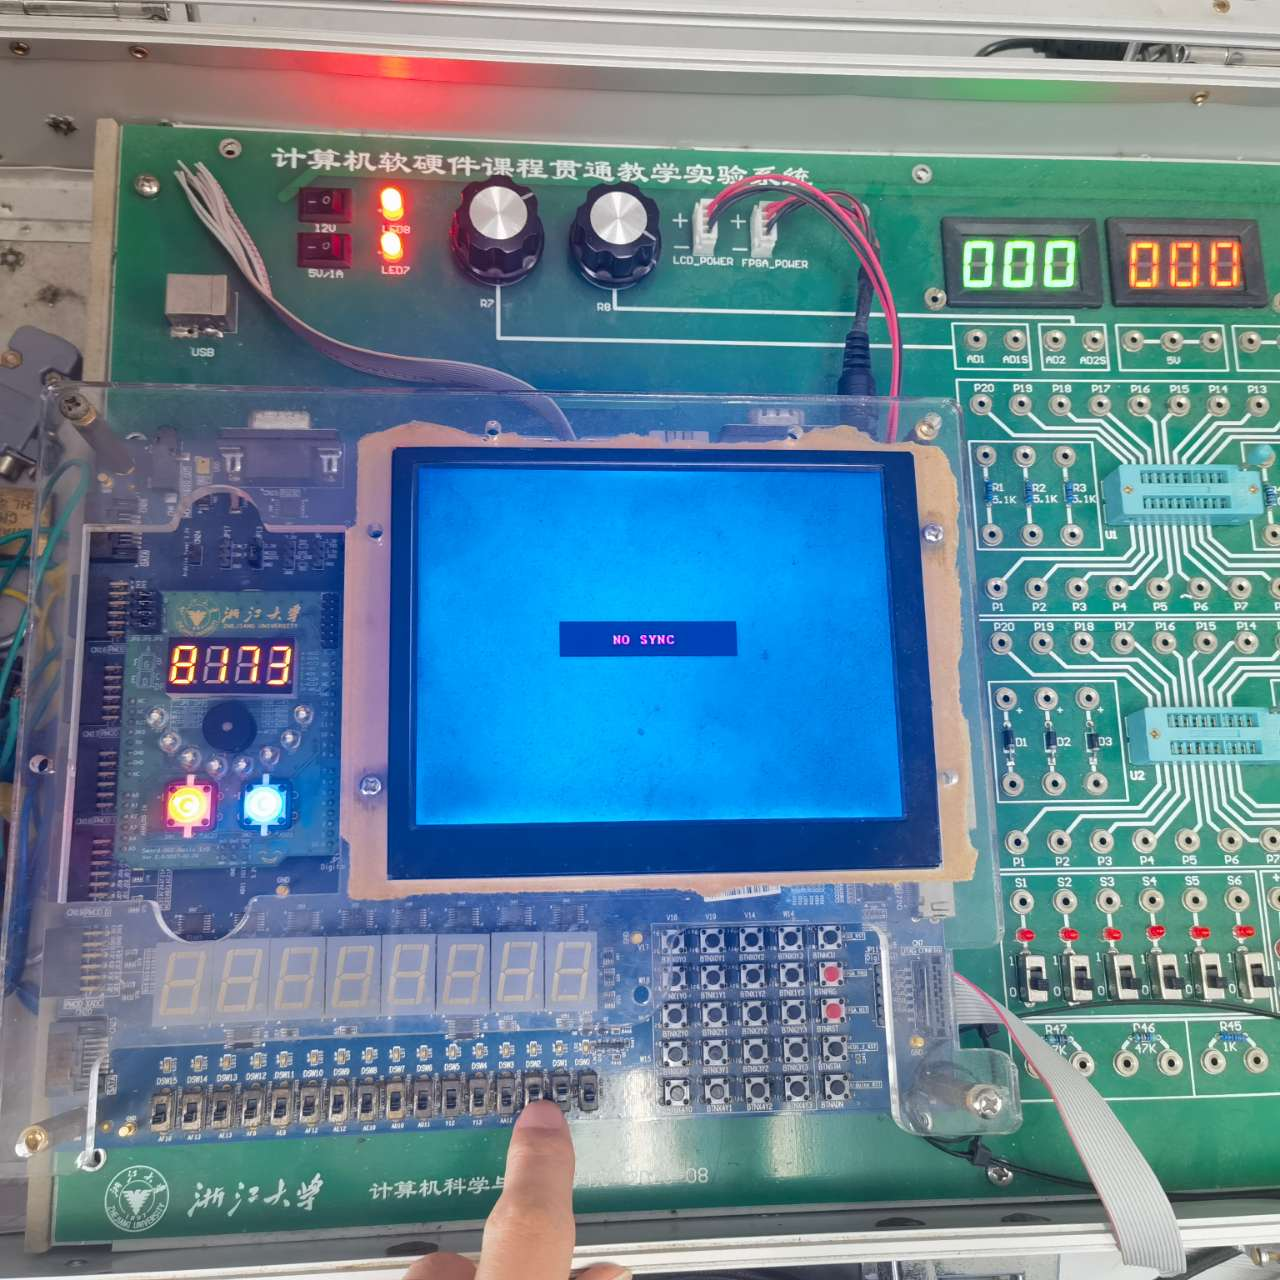
\includegraphics[width=0.5\textwidth]{3.jpg}
    \caption{\label{Lab11}下版验证:ALU}
    \end{figure}

    \begin{figure}[H]
    \centering
    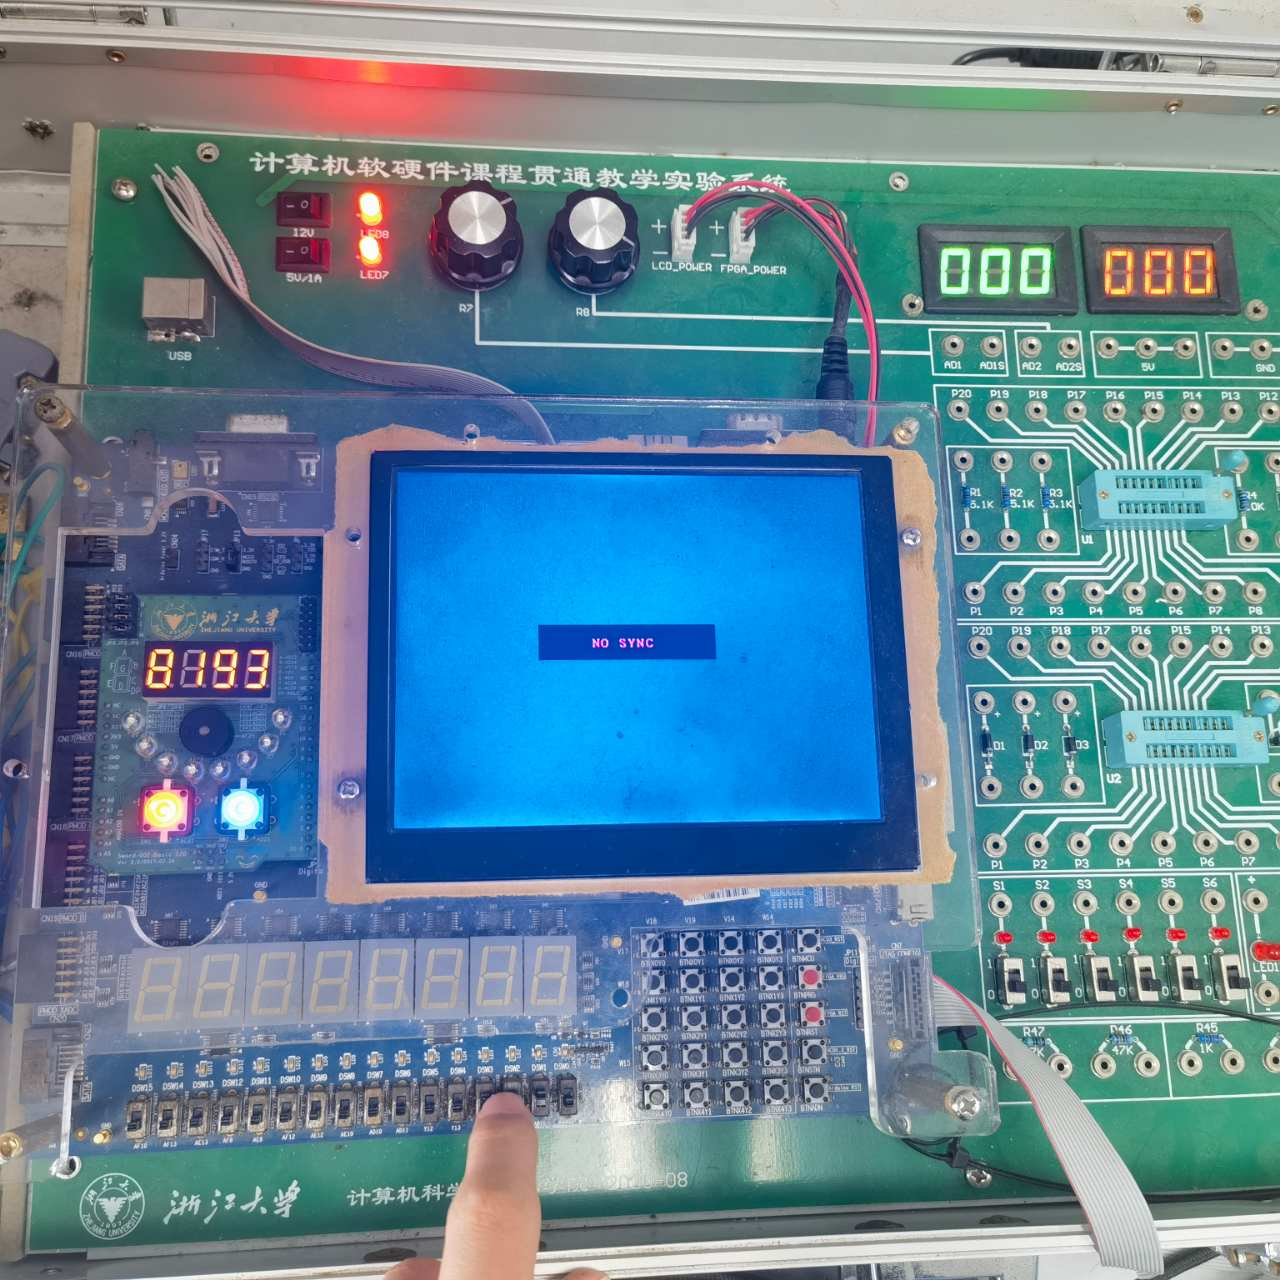
\includegraphics[width=0.5\textwidth]{4.jpg}
    \caption{\label{Lab11}下版验证:ALU}
    \end{figure}

    \begin{figure}[H]
    \centering
    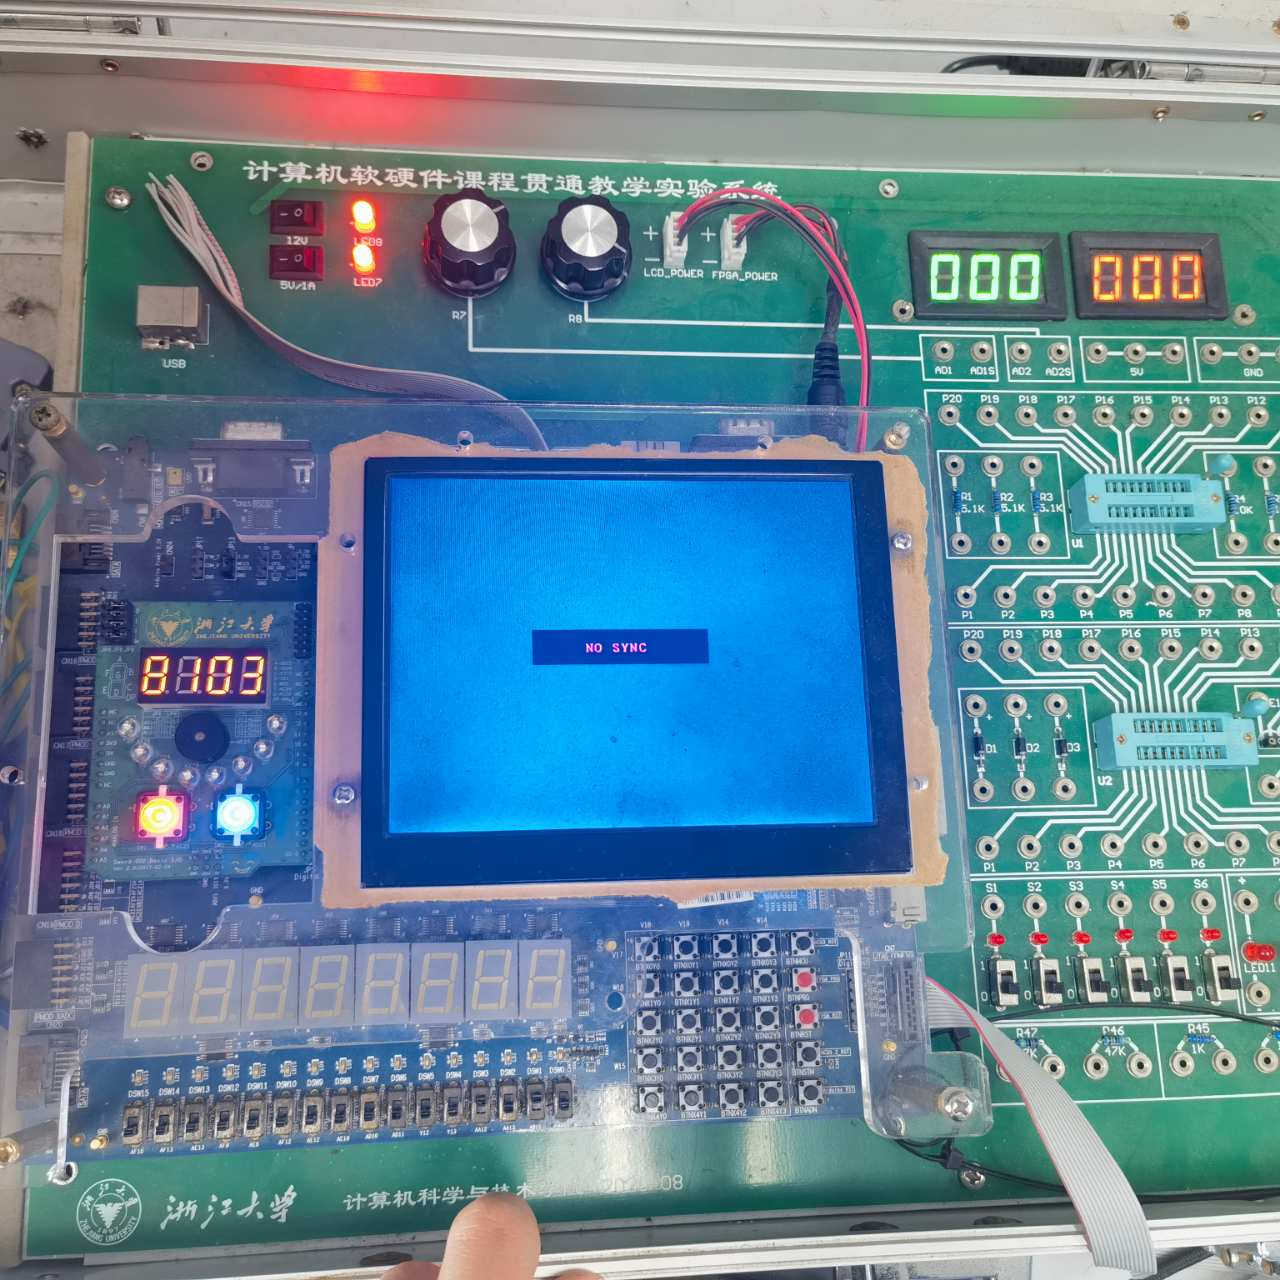
\includegraphics[width=0.5\textwidth]{5.jpg}
    \caption{\label{Lab11}下版验证:ALU}
    \end{figure}

    \begin{figure}[H]
    \centering
    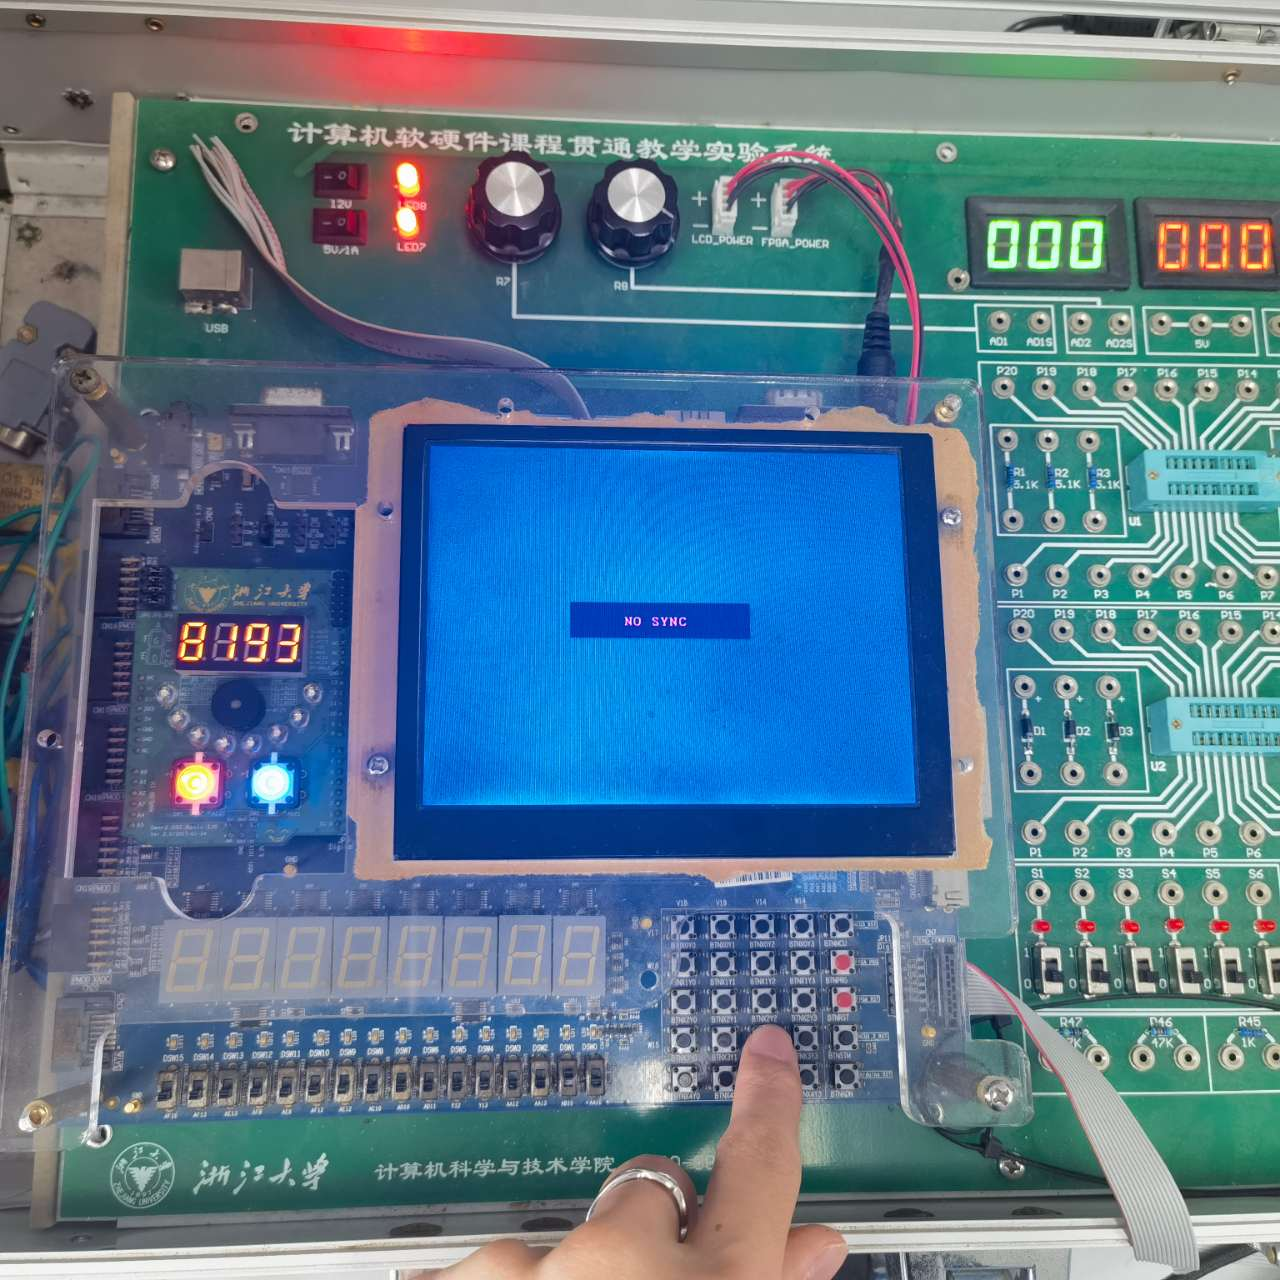
\includegraphics[width=0.5\textwidth]{6.jpg}
    \caption{\label{Lab11}下版验证:ALU}
    \end{figure}

    \begin{figure}[H]
    \centering
    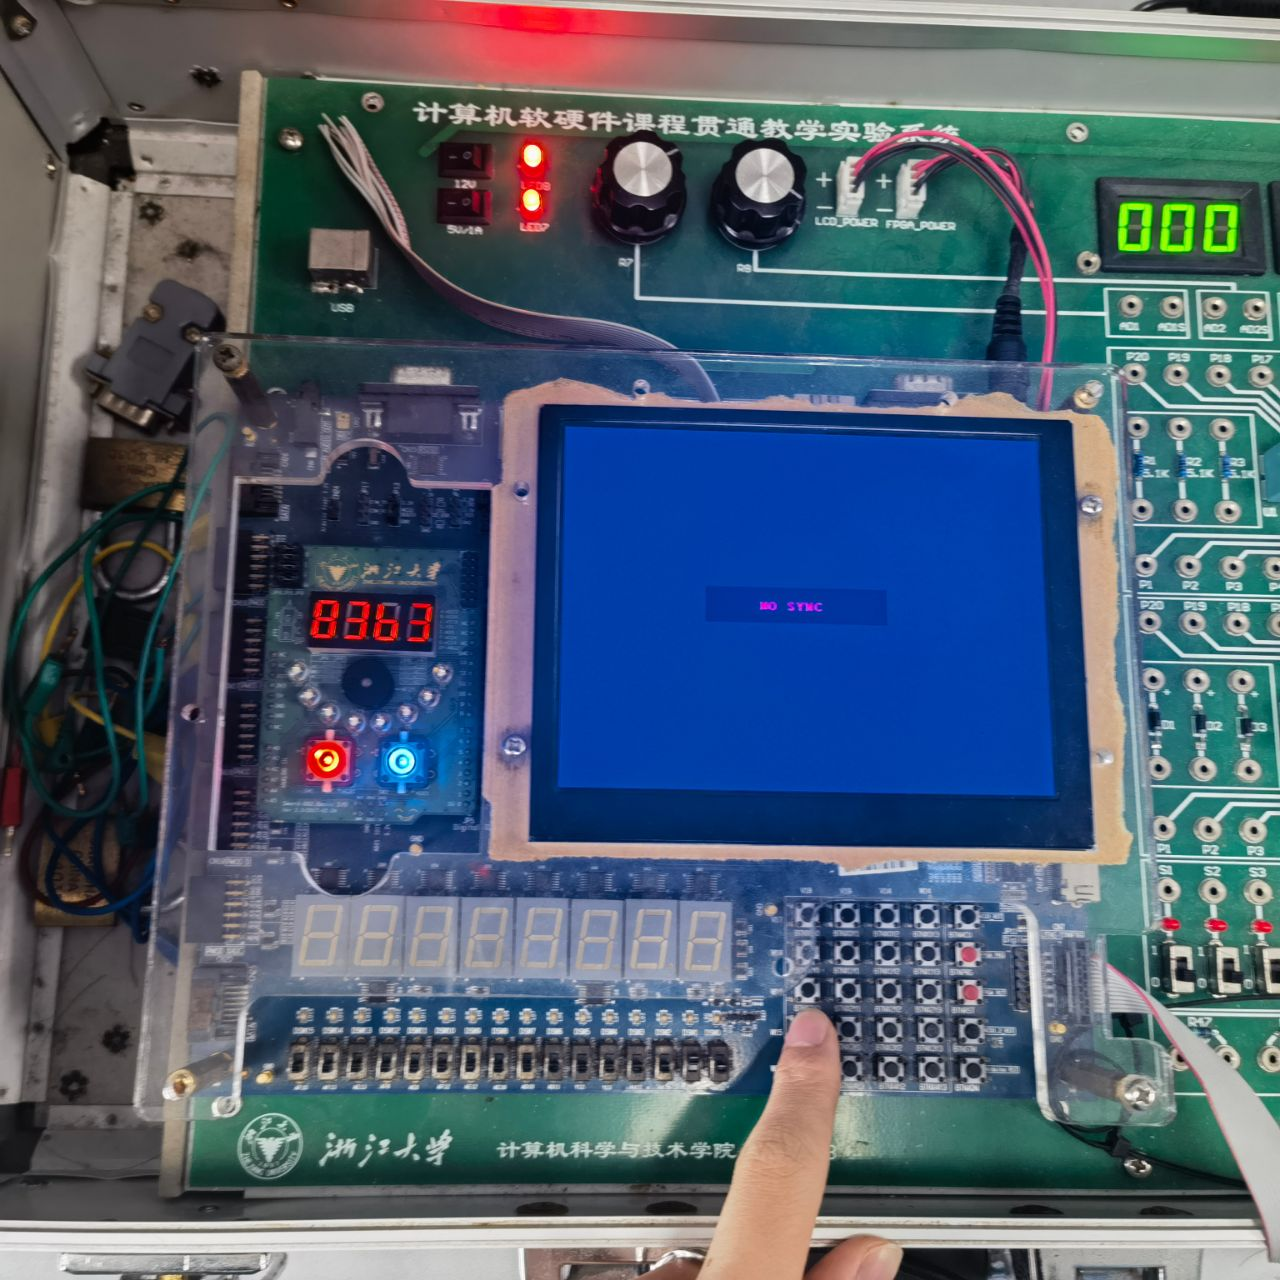
\includegraphics[width=0.5\textwidth]{7.jpg}
    \caption{\label{Lab11}下版验证:ALU}
    \end{figure}

    \begin{figure}[H]
    \centering
    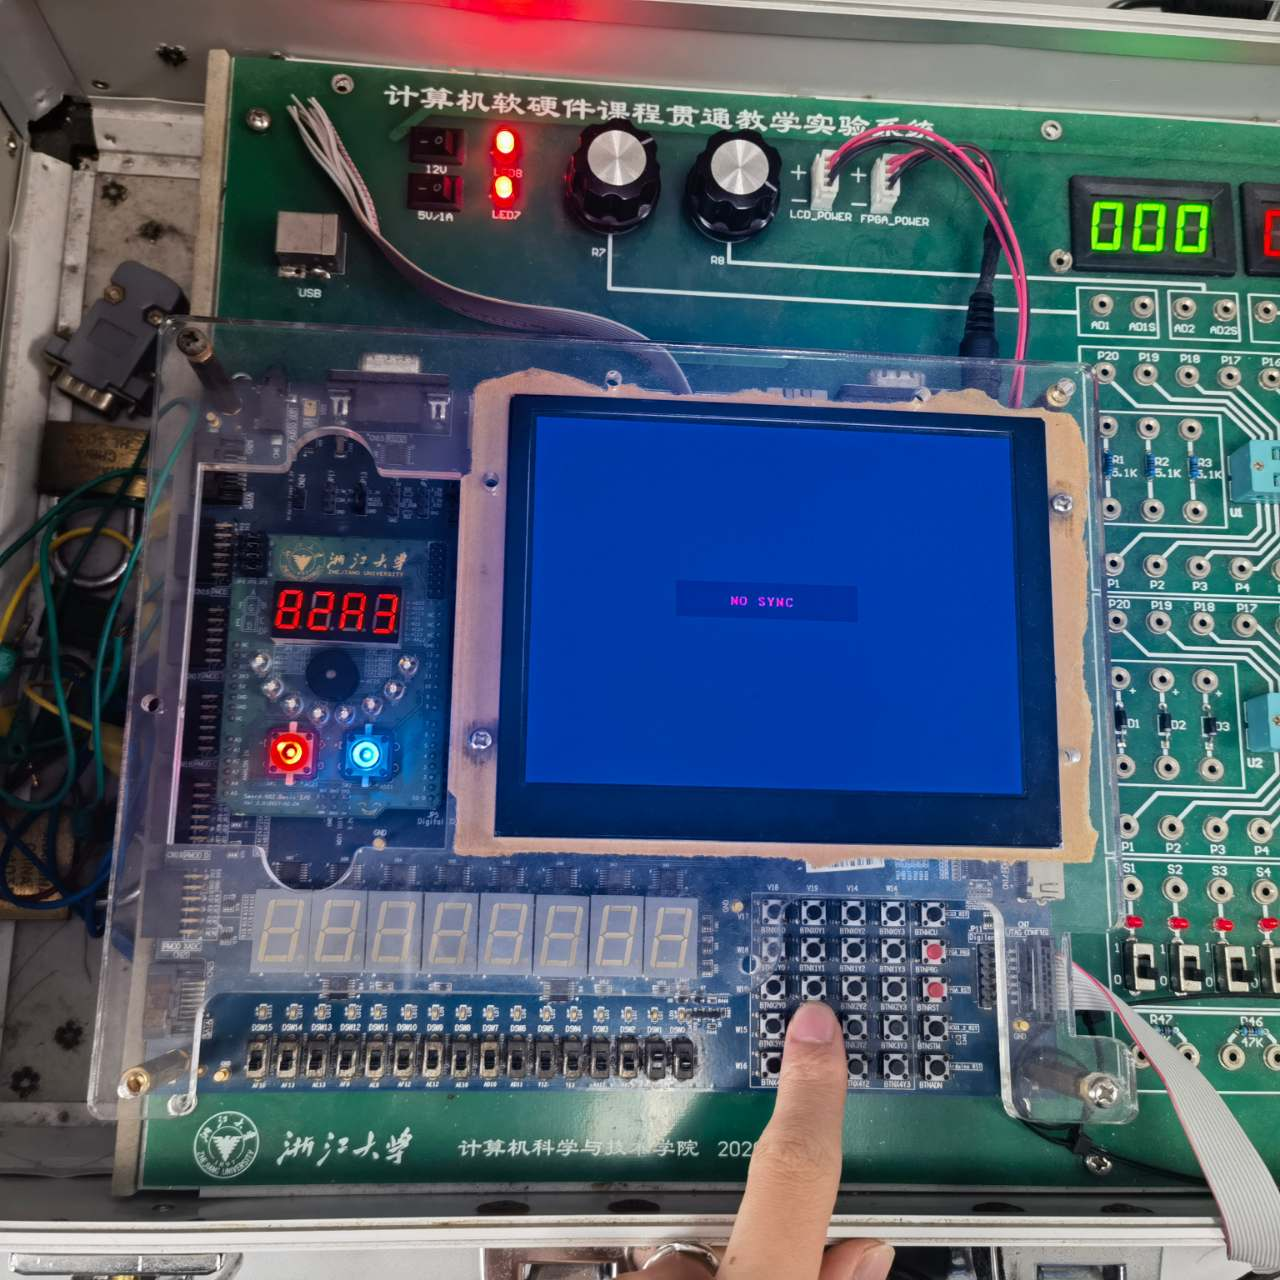
\includegraphics[width=0.5\textwidth]{8.jpg}
    \caption{\label{Lab11}下版验证:ALU}
    \end{figure}

    \begin{figure}[H]
    \centering
    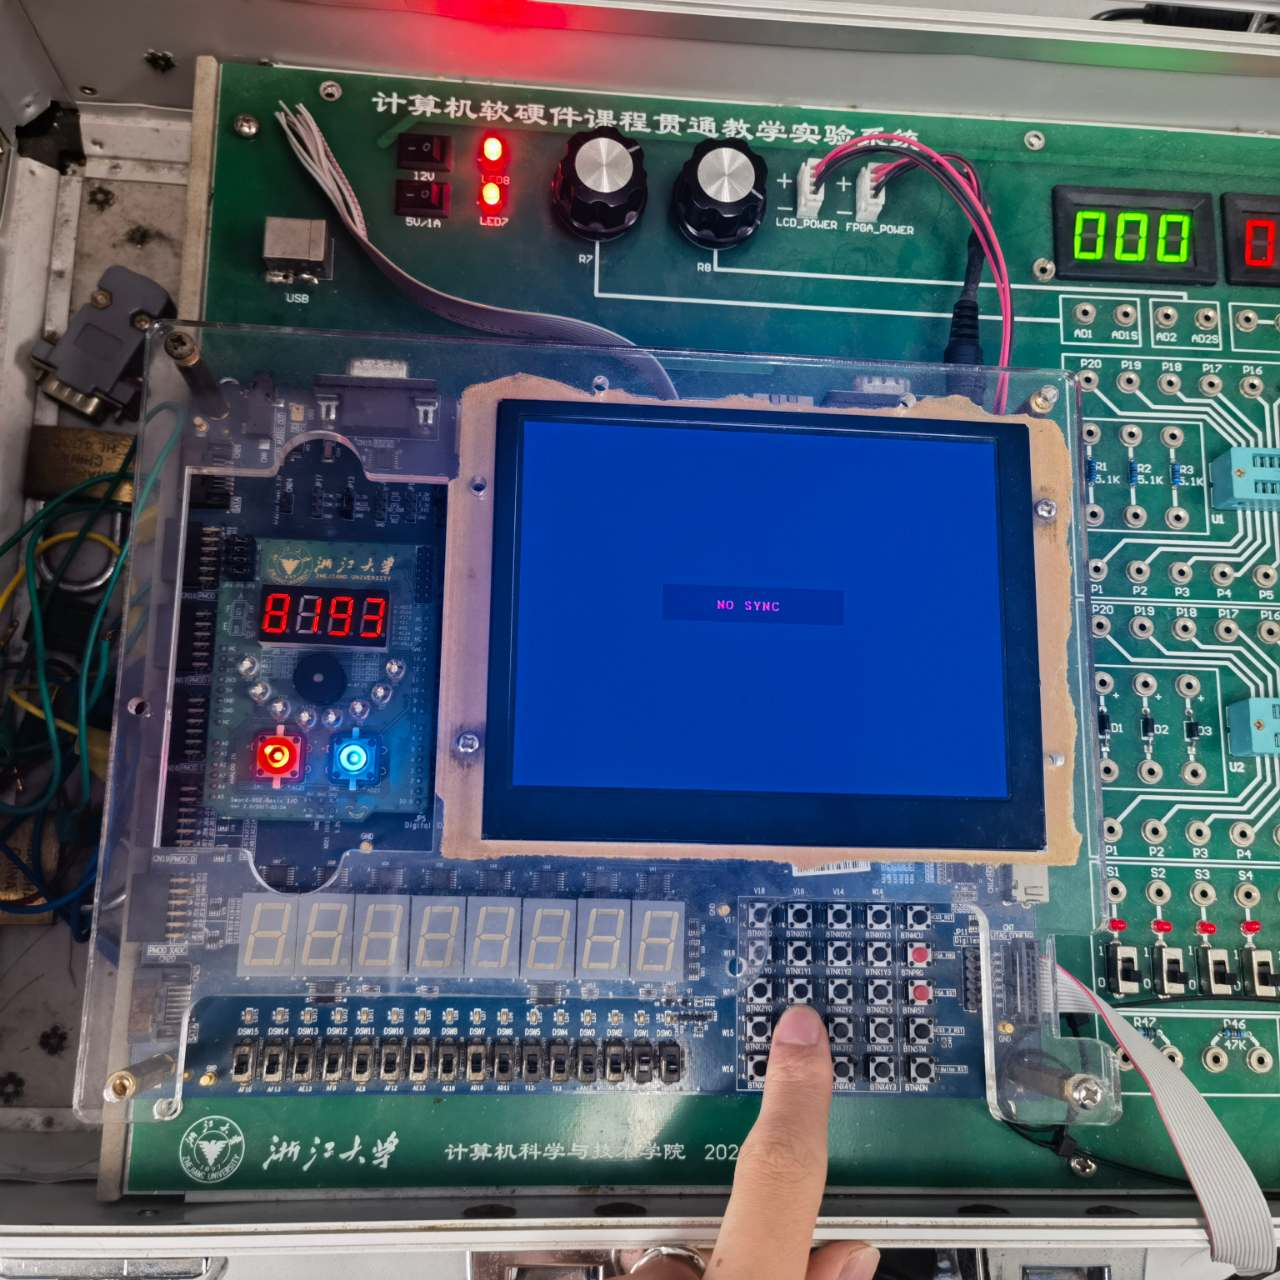
\includegraphics[width=0.5\textwidth]{9.jpg}
    \caption{\label{Lab11}下版验证:ALU}
    \end{figure}
    
\subsubsection*{ALU模式下版分析:}
数码管从左到右显示的四个数字分别是:寄存器A,寄存器B,ALU运算的结果,寄存器C所代表的数值.

控制sw[6:5]所对应的开关进行四种ALU运算,sw[6:5]为00时做加法,01做减法,
10做AND运算,11做OR运算,ALU运算时的两个操作数是A,B两个寄存器,运算得到的
结果显示在第三组数码管上.通过下板验证可以看出ALU运算的结果是正确的.

sw[0] 和 sw[1]控制寄存器A,B的自增和自减的运算,当按下对应的按钮后可以看到A,B两个寄存器
对应的数字发生了相应的变化.

\subsection*{数据传输模式:}
\subsubsection*{实验下版照片:}

    \begin{figure}[H]
    \centering
    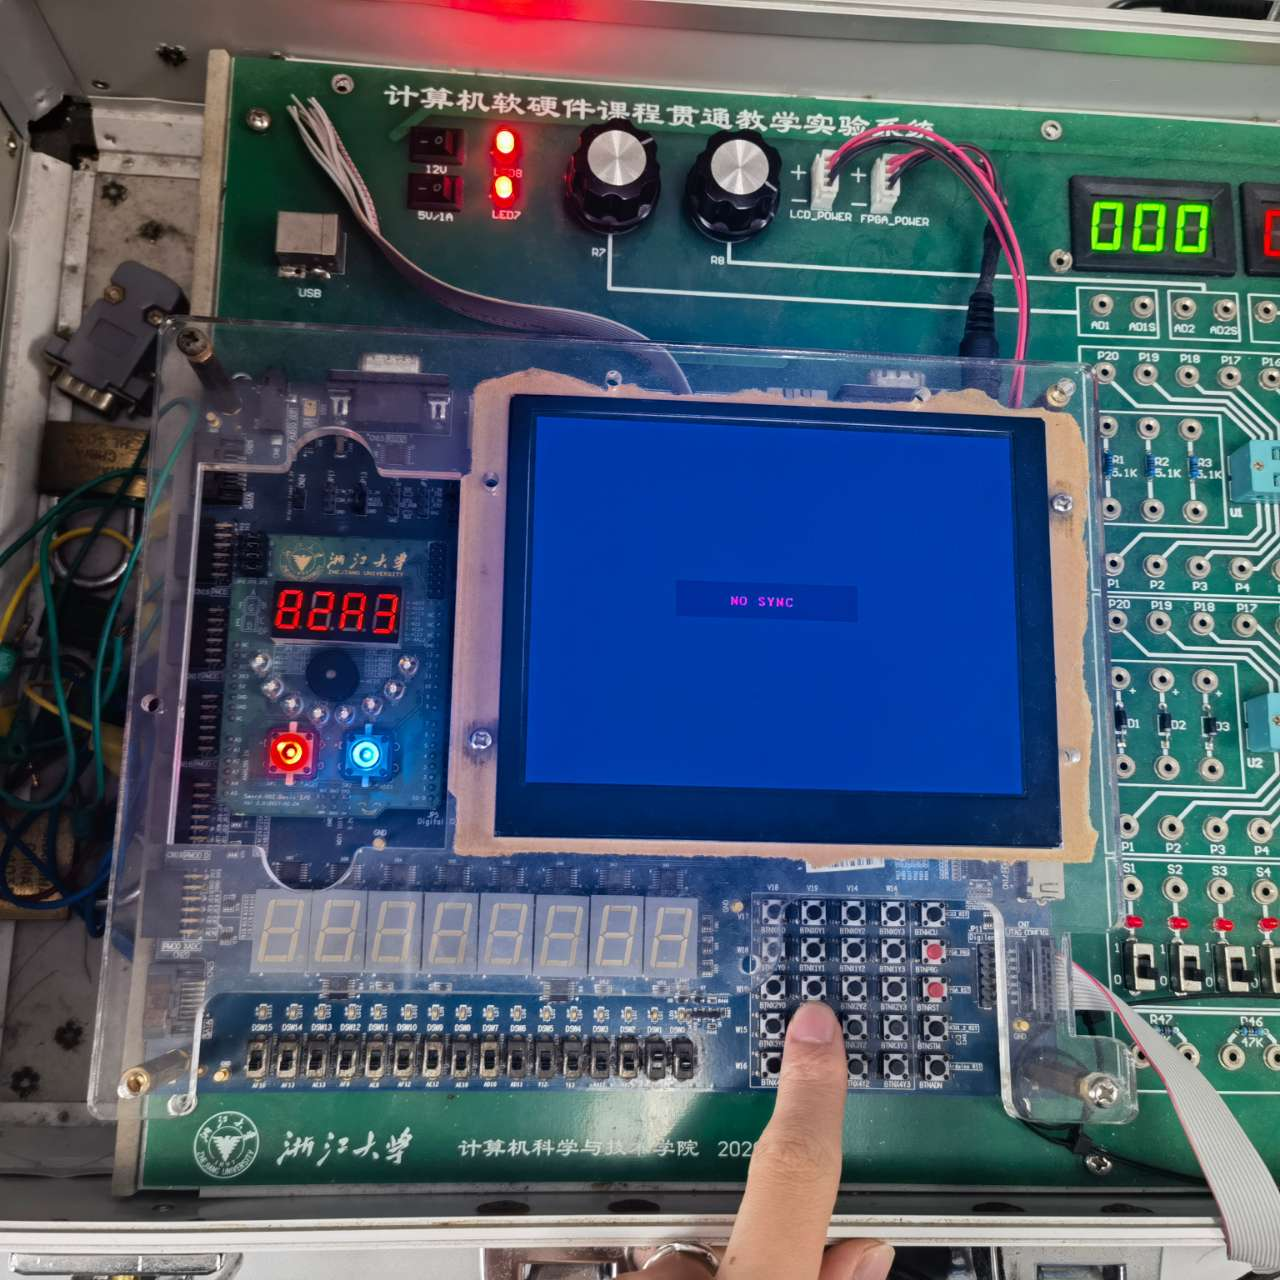
\includegraphics[width=0.5\textwidth]{11.jpg}
    \caption{\label{Lab11}下版验证:ALU}
    \end{figure}

    \begin{figure}[H]
    \centering
    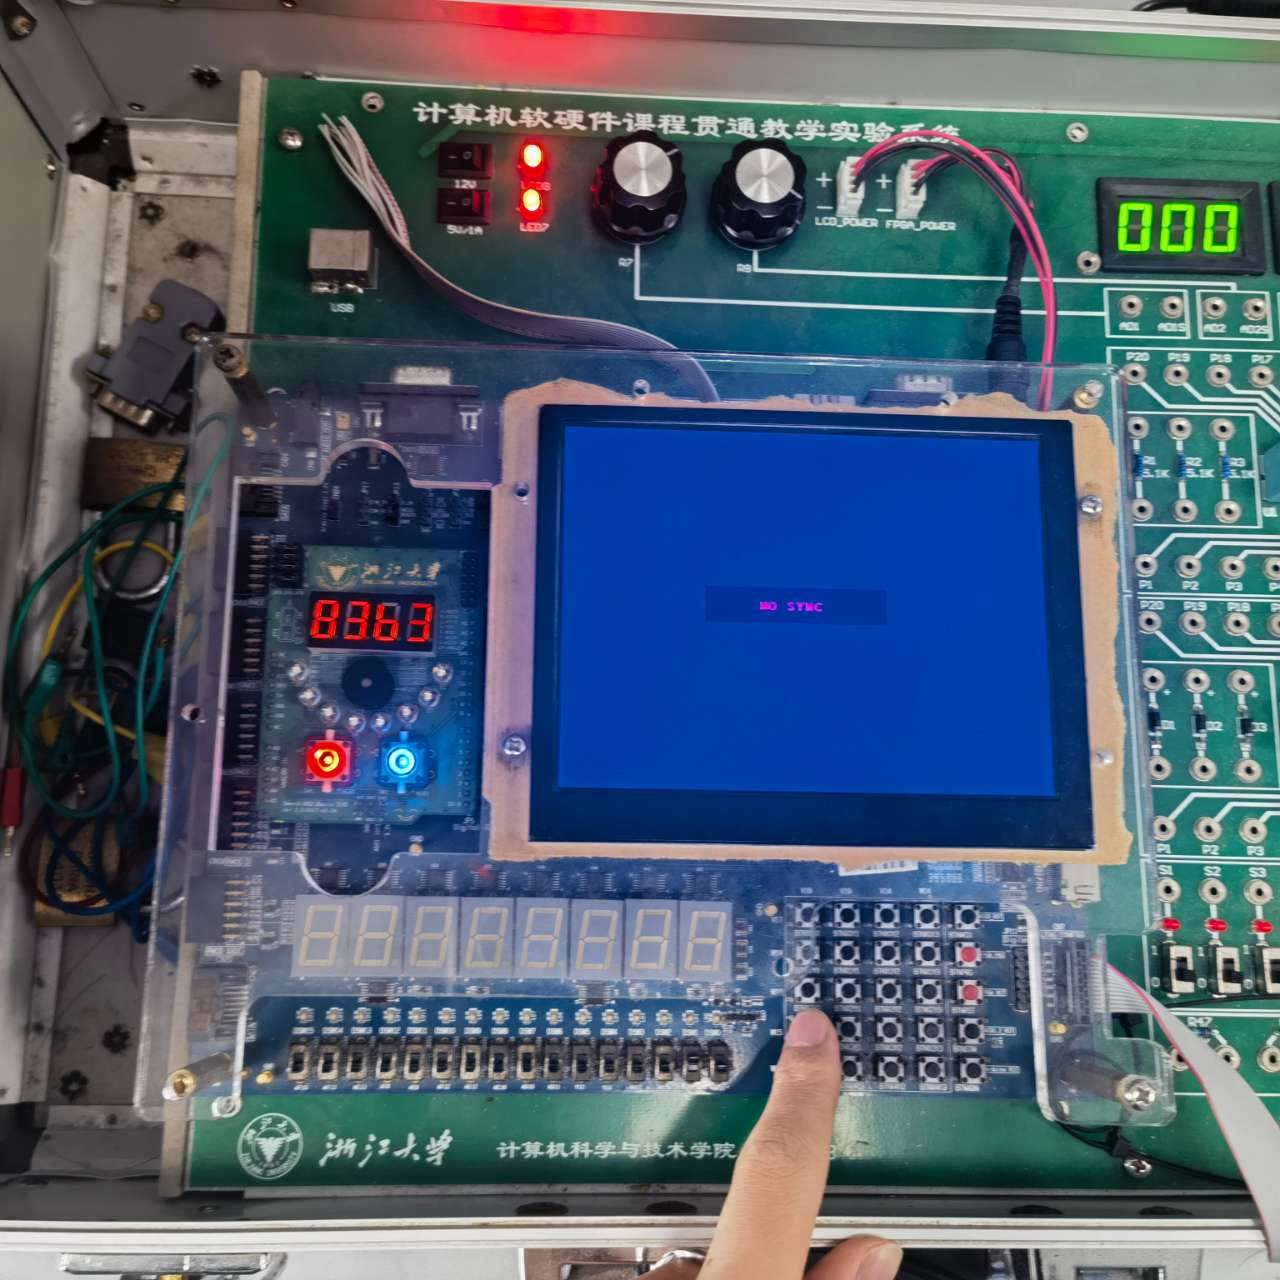
\includegraphics[width=0.5\textwidth]{10.jpg}
    \caption{\label{Lab11}下版验证:ALU}
    \end{figure}

    \begin{figure}[H]
        \centering
        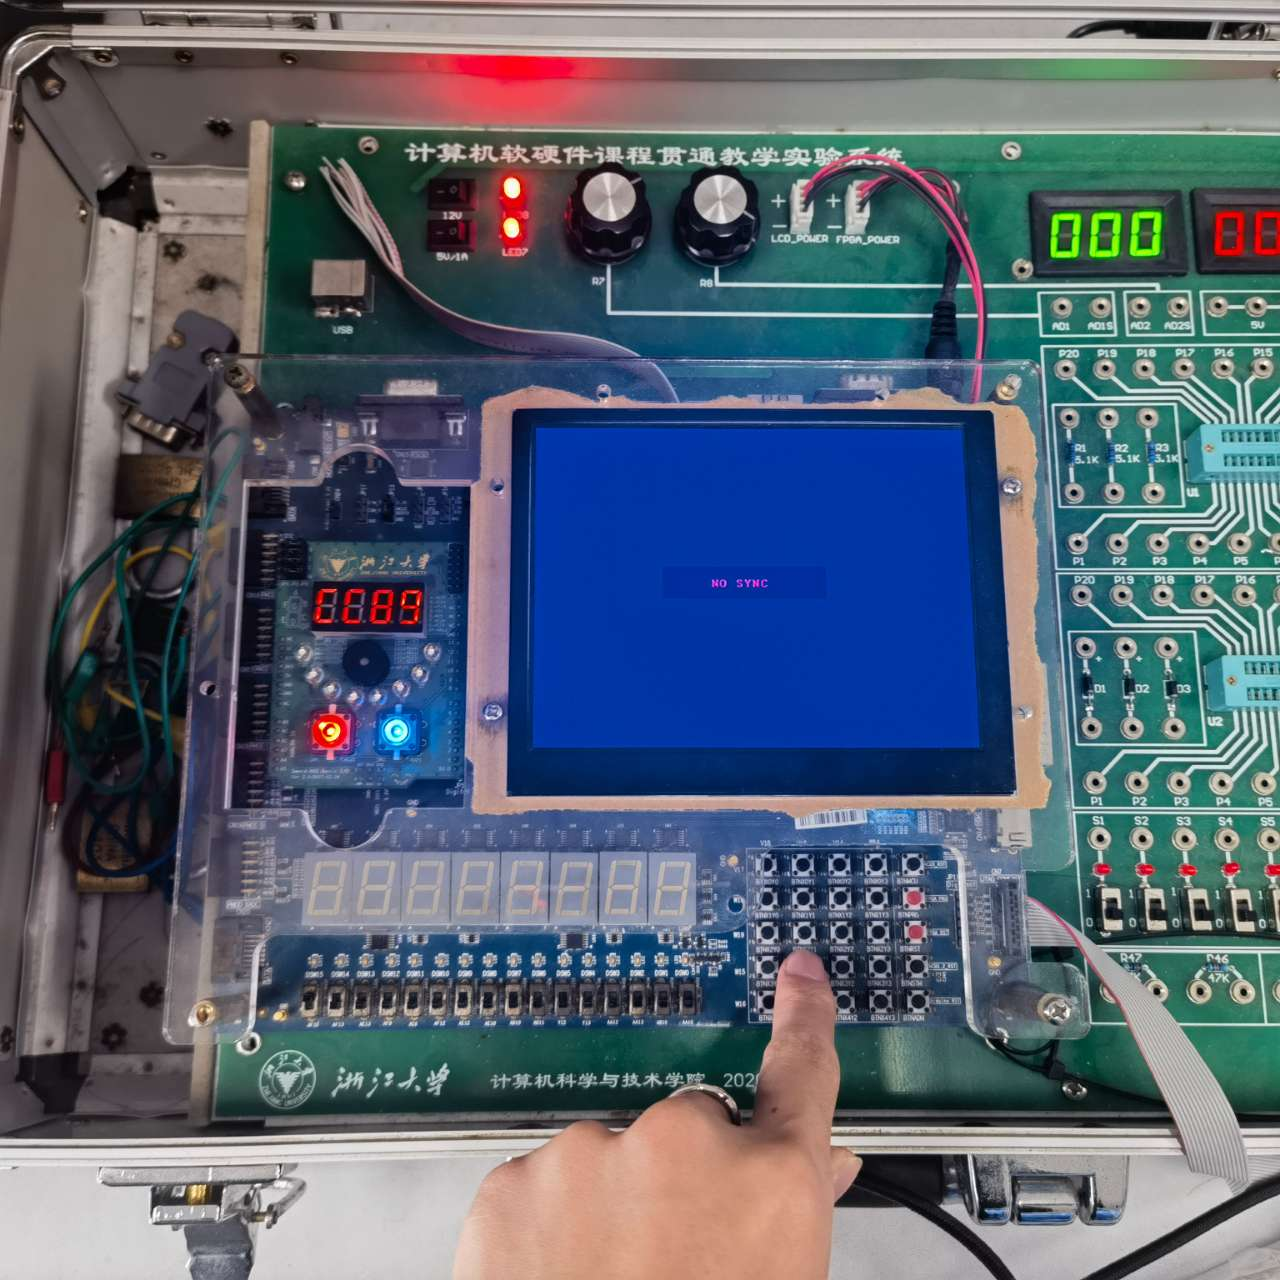
\includegraphics[width=0.5\textwidth]{12.jpg}
        \caption{\label{Lab11}下版验证:ALU}
        \end{figure}

    \begin{figure}[H]
        \centering
        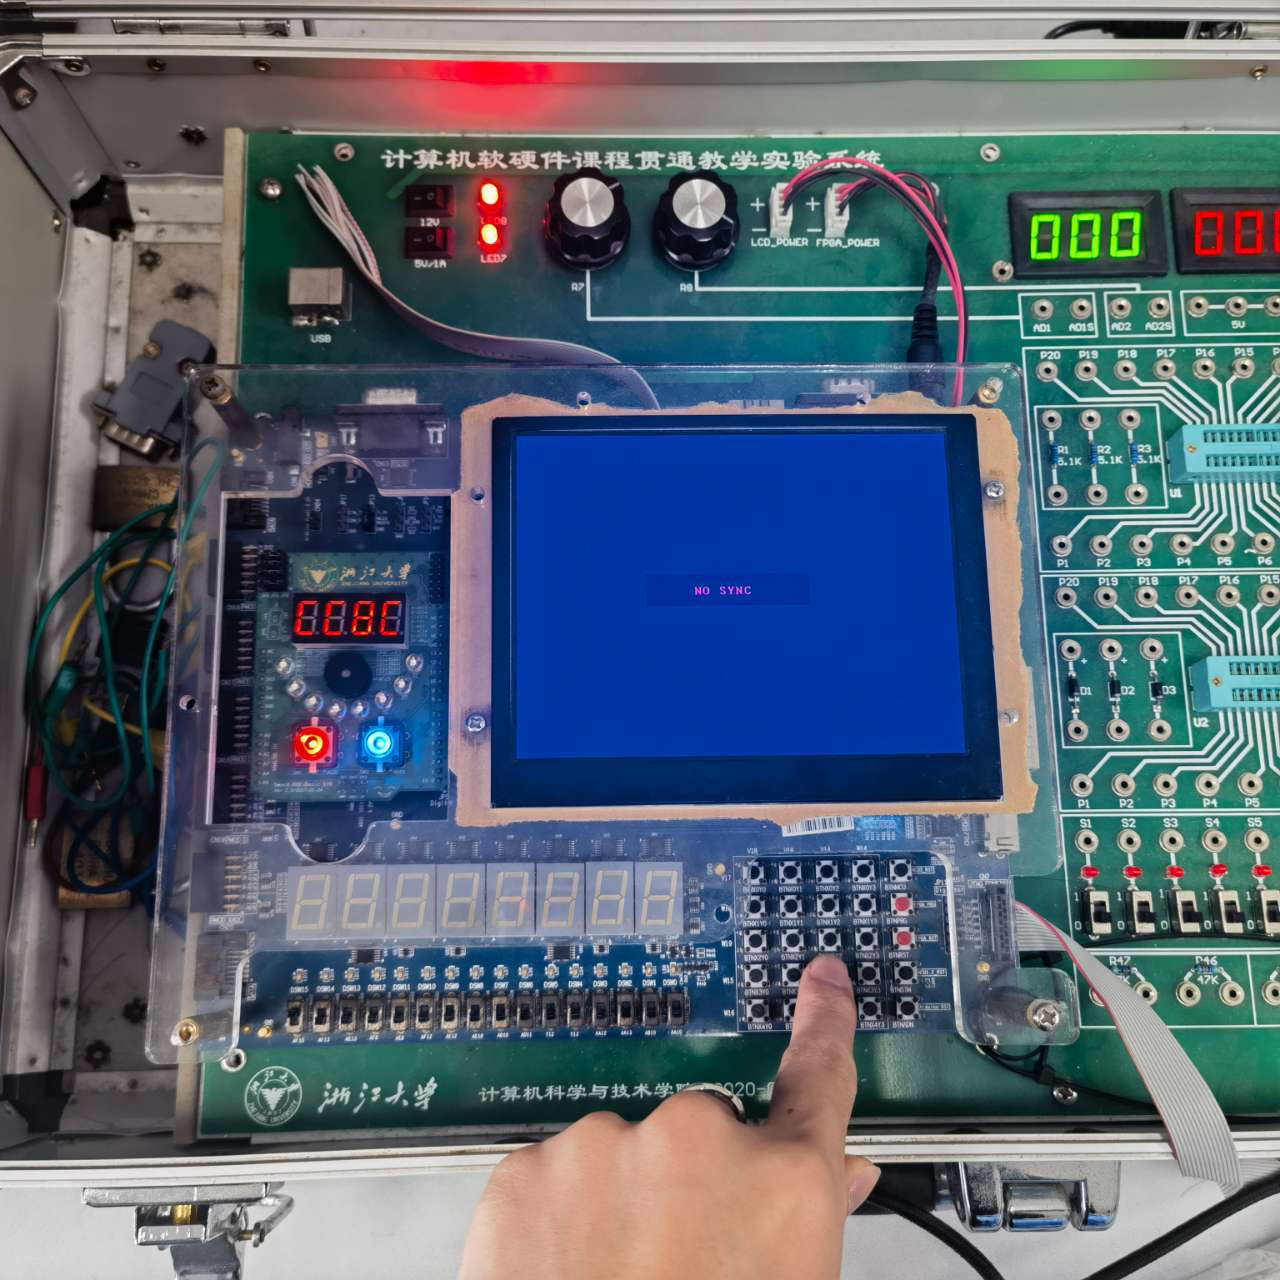
\includegraphics[width=0.5\textwidth]{13.jpg}
        \caption{\label{Lab11}下版验证:ALU}
        \end{figure}

\subsubsection*{传输模式结果分析:}
拨动开关使得SW[15]的信号为1,此时进入数据传输的模式.
SW[5:4]对要传输的数据进行选择,其中00选择A,01选择B,10选择C,11选择0,
然后通过按动寄存器绑定的三个按钮,可以将选择的数据进行传输,上面的前两张图为
寄存器C向寄存器B进行数据的传输.第3,4张图片为寄存器B向寄存器C进行的数据传输,
通过实际的下版分析可以验证这些功能都是正确的.



\section*{三、讨论与心得}
本次实验的内容主要与寄存器的传输和ALU运算相关,通过verilog语言实现了相应的功能,
本次实验主要遇到的问题是,实验课件的设计有些讲的不太清楚,刚开是自己做的时候对top.v的完成
有一些难度,后来借助助教提供的附件能够顺利完成,另外开始的top.v中ALU4b部分的填写给的有一些问题,
在下版时刚开始没有成功,对其进行修改后就顺利完成了实验.

\section*{四、Bonus:}
更新的testbench新增了在每次信号负边沿将BTN\_Y重新设定为0的操作,由于testbench
中的操作是在时钟正边沿进行触发的,如果不将BT\_Y重新设定为0,那么就会遇到信号1->1的情况,
但是由于边沿触发的条件,应当是0->1,才可以进行触发,否则验证就会存在一定问题,因此要做这样的修改.

\end{document}